\documentclass{scrreprt}
\usepackage{listings}
\usepackage{underscore}
\usepackage[bookmarks=true]{hyperref}
\usepackage[utf8]{inputenc}
\usepackage[english]{babel}

\usepackage{tcolorbox}
\usepackage{hyperref}

\hypersetup{
    bookmarks=false,    % show bookmarks bar?
    pdftitle={FP PROJECT REPORT},    % title
    pdfauthor={Saptarishi Dhanuka},                     % author
    pdfsubject={TeX and LaTeX},                        % subject of the document
    pdfkeywords={TeX, LaTeX, graphics, images}, % list of keywords
    colorlinks=true,       % false: boxed links; true: colored links
    linkcolor=blue,       % color of internal links
    citecolor=black,       % color of links to bibliography
    filecolor=black,        % color of file links
    urlcolor=purple,        % color of external links
    linktoc=page            % only page is linked
}%
\def\myversion{1.0 }
\date{}
%\title
\usepackage{hyperref}
\begin{document}

\begin{flushright}
    \rule{16cm}{5pt}\vskip1cm
    \begin{bfseries}
        \Huge{FUNCTIONAL PROGRAMMING \\ CS-IS-2010-1 \\ MIDTERM EVALUATION \\ PROJECT REPORT}\\
        \vspace{1.9cm}
        Haskell Web Scraper\\
        \vspace{1.9cm}
        Saptarishi Dhanuka\\
        \vspace{1.9cm}
        Ashoka University\\
    \end{bfseries}
\end{flushright}

\tableofcontents



\chapter{Problem Statement and Requirements}
\begin{tcolorbox}[colback=white,colframe=gray,title={Assigned Project Statement}]
    Develop a scraper using Haskell to extract text and code snippets separately.
    \begin{enumerate}
        \item \textbf{Input}: Scrape the text and code snippets from the given text \href{https://eli.thegreenplace.net/2018/type-erasure-and-reification/}{source}
        \item \textbf{Output}: A Word document containing the text and \texttt{.txt} file containing the code.
        \item \textbf{Method}: Write the algorithm to scrape (you can use the \texttt{tagsoup} library) and all the input-output facilities using Haskell. Do not use any other language.
    \end{enumerate}
\end{tcolorbox}

% in the design section can give the basic structure of the HTML page

\section{Problem Description}
The given web page is made of text and code snippets, which we need to scrape and extract separately into a \texttt{.docx} file containing the text portions and a \texttt{.txt} file which has the code snippets. \\ For this, we need to fetch the given web page, parse and analyze its HTML structure to identify the HTML tags of the code snippets and the tags of the rest of the text, so that we can effectively separate them into different documents.


\section{Requirements}

\begin{enumerate}
    \item The scraper shall be written entirely in Haskell
    \item The scraper shall get all text of the given page and write it into a \texttt{.docx} file.
    \item The scraper shall get all the code snippets of the given page and write it into a \texttt{.txt} file.
\end{enumerate}



% \begin{enumerate}
%     \item \textbf{Functional}
%     \begin{enumerate}
%         \item The scraper will be written entirely in Haskell
%         \item The scraper will accurately get all text of the given page and write it in a formatted manner into the \texttt{.txt} file. It will preserve the order and structure of the text on the page
%         \item The scraper will accurately get the code snippets of the given page and write it in ordered manner into a \texttt{.docx} file.
%     \end{enumerate}
    
%     \item \textbf{Non-functional}
%     \begin{enumerate}
%         \item The scraper will gracefully handle any errors that occur during it's running
%     \end{enumerate}
        
% \end{enumerate}



\chapter{Specifications}


\begin{enumerate}
    \item The scraper will use Haskell HTTP libraries for fetching the HTML content of the given web page.
    \item The scraper will separate the code snippets from the rest of the textual content using an algorithm that utilizes the \texttt{tagsoup} library to parse the HTML content, along with other standard libraries for string and text handling.
    \item The scraper will write the text into a Word document and the code snippets into a \texttt{.txt} file mainly using the \texttt{tagsoup} and \texttt{pandoc} libraries, along with some standard Haskell libraries.
    \item The \texttt{.txt} file will be formatted such that the code snippets are visibly delimited for readability purposes.
    \item The \texttt{.docx} file will be formatted in a mannger similar to the original web page in terms of demarcating headings, footnotes and the order of the text. 
    \item The scraper will handle errors gracefully.
\end{enumerate}




% \begin{enumerate}
%     \item \textbf{Limitations} % should limitations go here or later on cause it's seeming out of place here
%     % this can go in the design and architecture part or in the specs part
%     \begin{enumerate}
%         \item Since the HTML structure of different web pages can vary, it is not necessary that this particular scraper will work for all web pages. It is designed specifically for the given page and may work for some other pages. But no generalisation can be made about the correctness of its text and code extraction for other pages.
%         \item Moreover, it will not necessarily work for web pages with malformed HTML or different structure.
%         \item It is not designed to be robust to design changes, which is in line with the \href{https://hackage.haskell.org/package/tagsoup-0.6/src/tagsoup.htm#:~:text=Rule%202%3A%0ADo%20not%20be%20robust%20to%20design%20changes%2C%20do%20not%20even%20consider%20the%20possibility%20when%20writing%20the%20code.}{rule} stated on the \texttt{tagsoup} library's documentation example. If the site's HTML structure changes, for instance if the code snippets change from being enclosed in \texttt{<pre>} tags to \texttt{<code>} tags, then the scraper will not be able to separate out the code from the text and extract them accurately.
%     \end{enumerate}
% \end{enumerate}






\chapter{Design and Architecture}
% need to put functions into Lib and main stuff in main
% mention directory structure here along with basic ideas of the functions and code what it's doing


\section{High-Level Architecture}

% insert image here
\begin{figure}[h]
    \centering
    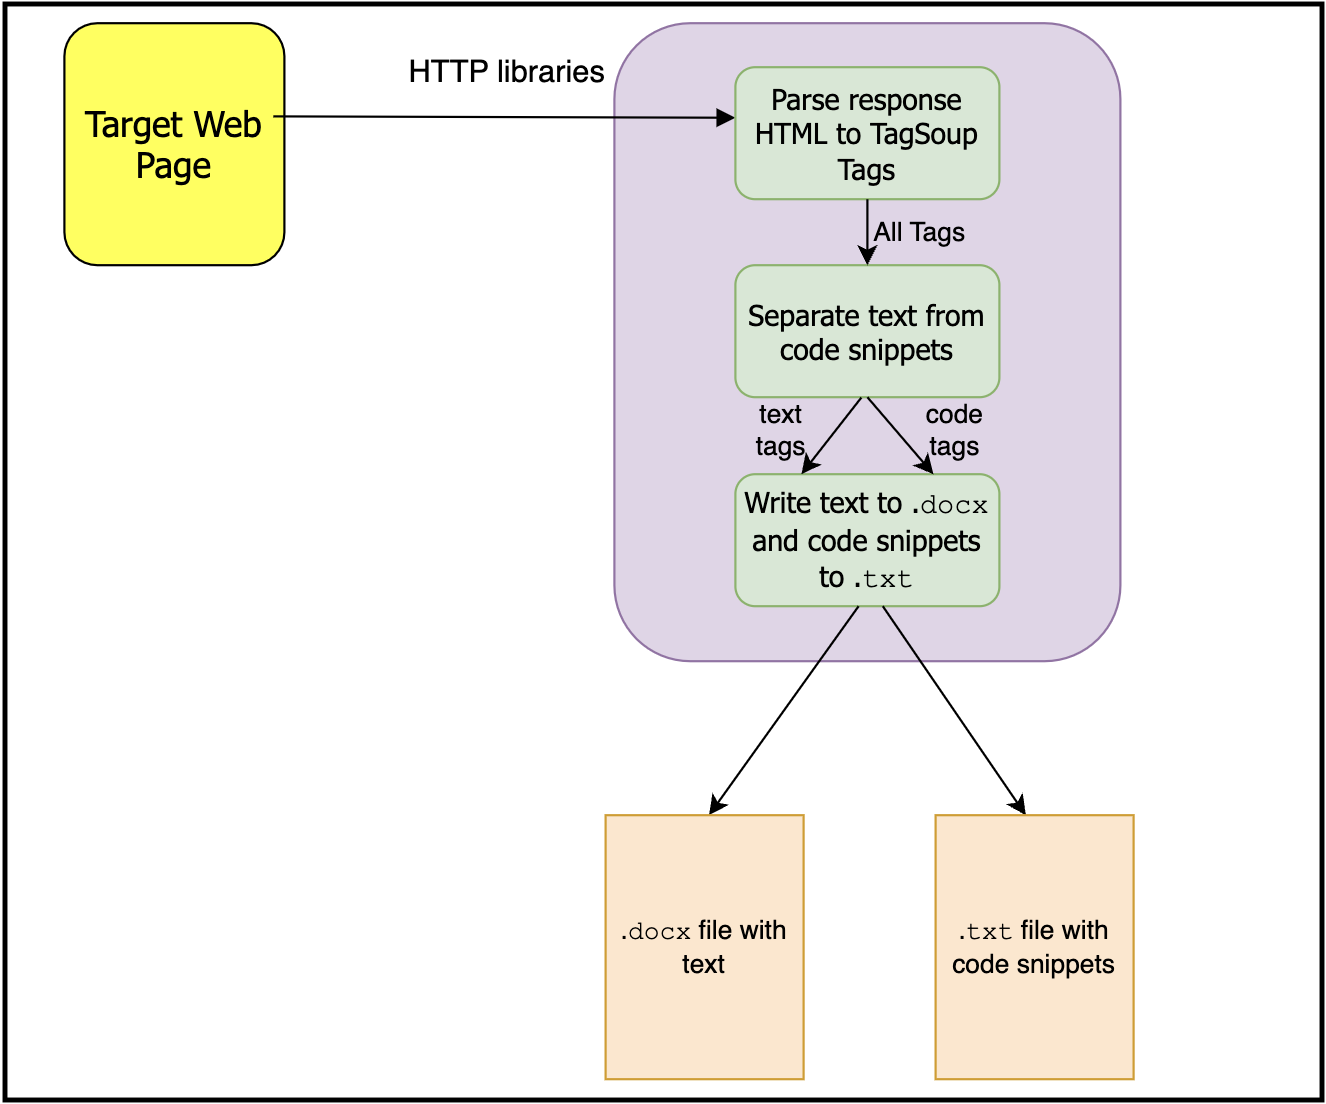
\includegraphics[width=0.8\textwidth]{figures/high-arch.png}
    \caption{High-Level Architecture}
    \label{fig:high-level-arch}
\end{figure}

The high level architecture consists of the following:
\begin{enumerate}
    \item Functionality for getting the target web page using HTTP libraries.
    \item Parsing the response obtained from the HTTP libraries into Tags from the \texttt{tagsoup} library.
    \item Separating the text from the code snippets using the descriptions of each Tag from the above Tags
    \item Extracting the visible content from the text tags and writing them into a \texttt{.docx} file
    \item Extracting the visible content from the code tags and writing them into a \texttt{.txt} file
\end{enumerate}

The high-level design which implements the above architecture consists of the following:
\begin{enumerate}
    \item 
\end{enumerate}











\chapter {Choice of Tools, Platforms, and Languages}
% tech stack
% need to be clear on cabal stack and haskell and stuff




\chapter{Test Plan}
% test individual functions 




\chapter{Prototype Implementation Details}
% what the prototype is outputting and stuff without formatting and stuff




\chapter{Plan for Completion}



















\end{document}